\documentclass{article}
\usepackage[margin=1in]{geometry}
\usepackage{problemset}
\showsolntrue

% Custom commands
\newcommand{\R}{\mathbb{R}}
\newcommand{\X}{\mathcal{X}}
\newcommand{\Y}{\mathcal{Y}}
\newcommand{\E}{\mathbb{E}}
\newcommand{\V}{\text{Var}}
\renewcommand{\P}{\mathbb{P}}

\begin{document}

\pstitle{%
    MATH 181A%
}{
    Homework 5%
}[due Thursday, February 12 at 11:59PM]

\begin{probset}

% --- Problem 1 ---
\begin{prob}
    Let $X_1, \dots , X_n$ be i.i.d. random variables from a Geometric($p$), $p \in (0, 1)$, which means that $P_X (k; p) = (1 - p)^{k-1}p$ for $k = 1, 2, \dots$ and we have $\E[X_i] = 1/p$.

    \begin{subprobset}
    \begin{subprob}
        Find the asymptotic variance of the maximum likelihood estimator $\hat{p}$.

        \begin{soln}
            The MLE is found as 
            \[
                \ell(p) = \sum_{i=1}^n \log \left( (1 - p)^{x_i - 1} p \right) = \sum_{i=1}^n (x_i - 1) \log(1 - p) + \sum_{i=1}^n \log p
            \]
            \[
                \frac{d}{dp} \ell(p) = -\sum_{i=1}^n \frac{x_i - 1}{1 - p} + \sum_{i=1}^n \frac{1}{p} = \frac{n}{1-p} - \frac{1}{1-p}\sum_{i=1}^n x_i + \frac{n}{p} = 0
            \]
            \[
                \frac{n}{1-p} - \frac{1}{1-p}\sum_{i=1}^n x_i + \frac{n}{p} = 0 \implies n - \sum_{i=1}^n x_i + \frac{n}{p} - n = 0 \implies \sum_{i=1}^n x_i = \frac{n}{p}
            \]
            \[
                \hat{p} = \frac{n}{\sum_{i=1}^n x_i} = \frac{1}{\bar{X}}
            \]
            The Fisher information is:
            \begin{align*}
                I(p) &= -\E\left[\frac{d^2}{dp^2} \log \left( (1 - p)^{X - 1} p \right) \right] \\
                &= -\E\left[\frac{d^2}{dp^2} (X - 1) \log(1 - p) + \log p \right] \\
                &= \E\left[\frac{(X - 1)}{(1 - p)^2} + \frac{1}{p^2} \right] = \frac{1 - p}{p(1 - p)^2} + \frac{1}{p^2} = \frac{1}{p^2(1-p)}
            \end{align*}
            Thus, the asymptotic variance of the MLE is:
            \[
                \V(\hat{p}) = \frac{1}{nI(\hat{p})} = \frac{p^2(1-p)}{n}
            \]
        \end{soln}
    \end{subprob}

    \begin{subprob}
        Let $n = 100$ and you observe the following data:
        
        \begin{center}
            \begin{tabular}{cccccc}
                \hline
                Number & 1 & 2 & 3 & 4 & 5 \\
                Frequency & 60 & 21 & 12 & 4 & 3 \\
                \hline
            \end{tabular}
        \end{center}

        which means that 60 of the random variables $X_1, \dots , X_{100}$ equal 1, 21 of them equal 2, and so on. Find a 95\% confidence interval for $p$ based on the MLE.

        \begin{soln}
            The MLE for $p$ is $\hat{p} = 1/\bar{X} = 1/1.69 \approx 0.5917$. The 95\% confidence interval for $p$ is:
            \[
                \hat{p} \pm z_{\alpha/2} \sqrt{\frac{1}{nI(\hat{p})}} = 0.5917 \pm 1.96 \sqrt{\frac{(0.5917)^2(1 - 0.5917)}{100}} = (0.5176, 0.6658)
            \]
        \end{soln}
    \end{subprob}
    \end{subprobset}
\end{prob}

\newpage

% --- Problem 2 ---
\begin{prob}
    Let $X_1, \dots , X_n$ be i.i.d. random variables from a $N (\sqrt{\mu}, 1)$ for $\mu \geq 0$. The MLE for $\mu$ is $\hat\mu = (\bar{X})^2$.

    \begin{subprobset}
    \begin{subprob}
        Find the (exact) variance of the MLE $\hat\mu$. Hint: You may use the fact that if $Y \sim N (\mu, \sigma^2)$, $\E[(Y - \mu)^4] = 3\sigma^4$.

        \begin{soln}
            \[
                \E[\bar{X}] = \E\left[\frac{1}{n} \sum_{i=1}^n X_i \right] = \frac{1}{n} \sum_{i=1}^n \E[X_i] = \frac{1}{n} \sum_{i=1}^n \sqrt{\mu} = \sqrt{\mu}
            \]
            \[
                \V(\bar{X}) = \frac{1}{n^2} \V\left(\sum_{i=1}^n X_i \right) = \frac{1}{n^2} \sum_{i=1}^n \V(X_i) = \frac{1}{n^2} \sum_{i=1}^n 1 = \frac{1}{n}
            \]
            \[
                \V(\hat\mu) = \V((\bar{X})^2) = \E[(\bar{X})^4] - (\E[(\bar{X})^2])^2
            \]
            \[
                \E[(\bar{X})^2] = \V(\bar{X}) + (\E[\bar{X}])^2 = \frac{1}{n} + (\sqrt{\mu})^2 = \frac{1}{n} + \mu
            \]
            Let $\bar{Z} \sim N(0, \frac{1}{n})$ then:
            \[
                \E[(\bar{X})^4] = \E[(\bar{Z} + \sqrt{\mu})^4] = \E[\bar{Z}^4 + 4\bar{Z}^3\sqrt{\mu} + 6\bar{Z}^2\mu + 4\bar{Z}\mu^{3/2} + \mu^2] = \frac{3}{n^2} + \frac{6\mu}{n} + \mu^2
            \]
            \[
                \V(\hat\mu) = \E[(\bar{X})^4] - (\E[(\bar{X})^2])^2 = \frac{3}{n^2} + \frac{6\mu}{n} + \mu^2 - \left(\frac{1}{n^2} + 2\frac{\mu}{n} + \mu^2\right) = \frac{2}{n^2} + \frac{4\mu}{n}
            \]
        \end{soln}
    \end{subprob}

    \begin{subprob}
        Find the asymptotic variance of the MLE $\hat\mu$.

        \begin{soln}
            The Fisher information is:
            \[
                I(\mu) = -\E\left[\frac{d^2}{d\mu^2} \log f_X(x; \mu)\right] = -\E\left[\frac{d}{d\mu} \frac{1}{2\sqrt{\mu}}(x - \sqrt{\mu}) \right] = \E\left[\frac{1}{4\mu}+\frac{1}{4\sqrt{\mu^{3}}}\left(x-\sqrt{\mu}\right) \right] = \frac{1}{4\mu}
            \]
            Thus, the asymptotic variance of the MLE is:
            \[
                \V(\hat\mu) = \frac{1}{nI(\hat\mu)} = \frac{4\mu}{n}
            \]
        \end{soln}
    \end{subprob}
    \end{subprobset}
\end{prob}

\newpage

% --- Problem 3 ---
\begin{prob}[\textbf{5.7.2}]
    Let $Y_1, Y_2, \dots, Y_n$ be a random sample of size $n$ from a normal pdf having $\mu = 0$. Show that $S^2_n = \frac{1}{n} \sum_{i=1}^n Y_i^2$ is a consistent estimator for $\sigma^2 = \V(Y)$. Hint: Likewise, you may use the fact that if $Y \sim N (0, \sigma^2)$, $\E(Y^4) = 3\sigma^4$.

    \begin{soln}
        \[
            \E[S^2_n] = \E\left[\frac{1}{n} \sum_{i=1}^n Y_i^2 \right] = \frac{1}{n} \sum_{i=1}^n \E[Y_i^2] = \frac{1}{n} \sum_{i=1}^n \V(Y_i) + (\E[Y_i])^2 = \frac{1}{n} \sum_{i=1}^n \sigma^2 + 0 = \sigma^2 \implies \text{unbiased}
        \]
        \[
            \V(S^2_n) = \V\left[\frac{1}{n} \sum_{i=1}^n Y_i^2 \right] = \frac{1}{n^2} \V\left[\sum_{i=1}^n Y_i^2 \right] = \frac{1}{n^2} \sum_{i=1}^n \V(Y_i^2)
        \]
        \[
            = \frac{1}{n^2} \sum_{i=1}^n \E[Y_i^4] - \left(\E[Y_i^2]\right)^2 = \frac{1}{n^2} \sum_{i=1}^n 3\sigma^4 - \sigma^4 = \frac{2\sigma^4}{n}
        \]
        Since $\lim_{n \to \infty} \V(S^2_n) = 0$ then $S^2_n$ is a consistent estimator for $\sigma^2$.
    \end{soln}
\end{prob}

% --- Problem 4 ---
\begin{prob}
    Let $Y_1, Y_2, \dots, Y_n$ be a random sample of size $n$ from the pdf $f_Y(y; \theta) = \frac{1}{\theta} e^{-y/\theta}, y > 0$. Let $\hat\theta_1 = Y_1$, $\hat\theta_2 = \bar Y$, and $\hat\theta_3 = n \cdot Y_{\min}$ Show if each of the estimators is consistent for $\theta$ or not. You can use some of the results you have done in Homework 4 Problem 1.

    \begin{soln}
        We know from HW 4 1.1 that they are all unbiased estimators for $\theta$. We also know the variances from HW 4 1.2 with $\V(\hat\theta_1) = \V(\hat\theta_3) = \theta^2$, $\V(\hat\theta_2) = \theta^2/n$. Hence the only estimator that is consistent for $\theta$ is $\hat\theta_2$ since $\lim_{n \to \infty} \V(\hat\theta_2) = 0$ while $\lim_{n \to \infty} \V(\hat\theta_1) = \lim_{n \to \infty} \V(\hat\theta_3) = \theta^2 \neq 0$.
    \end{soln}
\end{prob}

\newpage

% --- Problem 5 ---
\begin{prob}
    Suppose $\hat\theta_n = Y_{\max}$ is to be used as an estimator for the parameter $\theta$ in the uniform pdf, $f_Y(y; \theta) = 1/\theta, 0 \leq y \leq \theta$. Show that $\hat\theta_n$ is squared-error consistent (see Question 5.7.4).

    \begin{soln}
        $\hat\theta_n$ is squared-error consistent if $\lim_{n \to \infty} \E[(\hat\theta_n - \theta)^2] = 0$. First, we'll need the first and second moments of $Y_{\max}$.

        \[
            \P(Y_{\max} \leq y) = \P(Y_1 \leq y, \dots, Y_n \leq y) = \P(Y_1 \leq y)^n = \left(\frac{y}{\theta}\right)^n
        \]
        \[
            f_{Y_{\max}}(y) = \frac{d}{dy} \P(Y_{\max} \leq y) = \frac{d}{dy} \left(\frac{y}{\theta}\right)^n = n\left(\frac{y}{\theta}\right)^{n-1} \cdot \frac{1}{\theta} = \frac{n}{\theta} \left(\frac{y}{\theta}\right)^{n-1}
        \]
        \[
            \E[Y_{\max}] = \int_0^\theta y \frac{n}{\theta} \left(\frac{y}{\theta}\right)^{n-1} dy = \frac{n}{\theta^n} \int_0^\theta y^n dy = \frac{n}{\theta^n} \left[\frac{y^{n+1}}{n+1}\right]_0^\theta = \frac{n}{\theta^n} \cdot \frac{\theta^{n+1}}{n+1} = \frac{n\theta}{n+1}
        \]
        \[
            \E[Y_{\max}^2] = \int_0^\theta y^2 \frac{n}{\theta} \left(\frac{y}{\theta}\right)^{n-1} dy = \frac{n}{\theta^n} \int_0^\theta y^{n+1} dy = \frac{n}{\theta^n} \left[\frac{y^{n+2}}{n+2}\right]_0^\theta = \frac{n}{\theta^n} \cdot \frac{\theta^{n+2}}{n+2} = \frac{n\theta^2}{n+2}
        \]
        \[
            \E[(\hat\theta_n - \theta)^2] = \E[(Y_{\max} - \theta)^2] = \E[Y_{\max}^2] - 2\theta\E[Y_{\max}] + \theta^2 = \frac{n\theta^2}{n+2} - \frac{2n\theta^2}{n+1} + \theta^2 = \frac{2\theta^2}{n^2+3n+2}
        \]
        Since $\lim_{n \to \infty} \E[(\hat\theta_n - \theta)^2] = 0$ then $\hat\theta_n$ is squared-error consistent.
    \end{soln}
\end{prob}

% --- Problem 6 ---
\begin{prob}
    Suppose $X_1, X_2, \dots$ is a sequence of i.i.d. random variables having the Poisson distribution with mean $\lambda$. Let $\hat\lambda_n = X_n$ (the last random variable).

    \begin{subprobset}
    \begin{subprob}
        Is $\hat\lambda_n$ an unbiased estimator of $\lambda$? Explain your answer.

        \begin{soln}
            Yes, since $\E[\hat\lambda_n] = \E[X_n] = \E[X_i] = \lambda$.
        \end{soln}
    \end{subprob}

    \begin{subprob}
        Is $\hat\lambda_n$ a consistent estimator of $\lambda$? Explain your answer.

        \begin{soln}
            No, since $\V(\hat\lambda_n) = \V(X_n) = \V(X_i) = \lambda$. Hence $\lim_{n \to \infty} \V(\hat\lambda_n) = \lambda \neq 0$.
        \end{soln}
    \end{subprob}
    \end{subprobset}
\end{prob}

\newpage

% --- Problem 7 ---
\begin{prob}[\textbf{R Simulation}]
    \begin{subprobset}
    \begin{subprob}
        For $n = 1000$, simulate a random sample of size $n$ from $N (0, 1)$. Use the generated data to give an approximation to the critical values when $\alpha = 0.01, 0.05, 0.1$, and compare them with the theoretical values $z_{\alpha/2}$. Repeat with $n = 10, 000$ to get a better approximation. Hint: Commands \texttt{quantile()}, \texttt{qnorm()} may be helpful.

        \begin{verbatim}
[1] "Theoretical z_{alpha/2}:"
alpha=0.01 alpha=0.05  alpha=0.1
    2.5758     1.9600     1.6449
[1] "Approximation (n = 1000):"
alpha=0.01 alpha=0.05  alpha=0.1
    2.7020     1.8777     1.5335
[1] "Difference from theoretical:"
alpha=0.01 alpha=0.05  alpha=0.1
    0.1262    -0.0823    -0.1114
[1] "Approximation (n = 10000):"
alpha=0.01 alpha=0.05  alpha=0.1
    2.5533     1.9611     1.6619
[1] "Difference from theoretical:"
alpha=0.01 alpha=0.05  alpha=0.1
   -0.0225     0.0011     0.0171
        \end{verbatim}

        \begin{soln}
            The differences are about an order of magnitude smaller for $n = 10000$ compared to $n = 1000$ which is expected since more data is being used.
        \end{soln}
    \end{subprob}

    \begin{subprob}
        For $n = 10$, simulate a random sample of size $n$ from $N (\mu, \sigma^2)$, where $\mu = 1$ and $\sigma^2 = 2$; compute the sample mean. Repeat the above simulation 500 times, plot the histogram of the 500 sample means. Now repeat the 500 simulations for $n = 1, 000$. Compare these two sets of results with different sample sizes, and discuss it in the context of consistency.

        \begin{soln}
            \begin{center}
                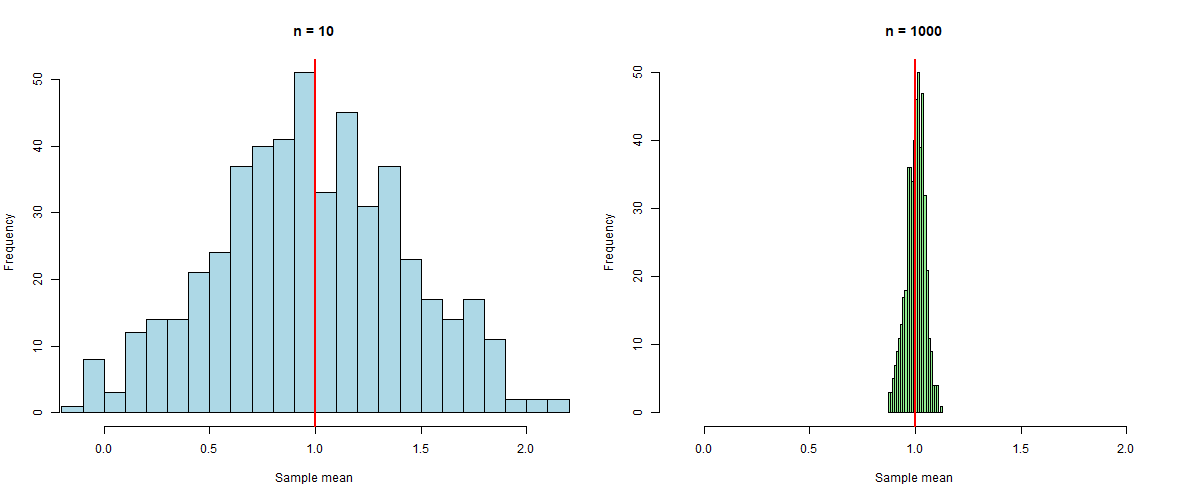
\includegraphics[width=0.8\textwidth]{Images/7.2.png}
            \end{center}
            The $n = 1000$ histogram is much more concentrated around the mean of 1, while the $n = 10$ histogram is more spread out. This is expected since the variance of the sample mean is $\frac{\sigma^2}{n}$ and the variance of the sample mean of $n = 1000$ is much smaller than the variance of the sample mean of $n = 10$.

            We know that the sample mean is a consistent estimator for the mean of the distribution, so as $n$ increases, the sample mean will converge to the true mean. Hence, the histogram of the sample means will be more concentrated around the true mean.
        \end{soln}
    \end{subprob}
    \end{subprobset}
\end{prob}
\end{probset}
\end{document}
